\begin{aosachapter}{ITK}{s:itk}{Luis Ib\'{a}\~{n}ez and Brad King}

%% American spelling 

\begin{aosasect1}{What Is ITK?}
ITK (the Insight Toolkit)\footnote{\url{http://www.itk.org}} is a library for
image analysis that was developed by the initiative, and mainly with the
funding, of the US National Library of
Medicine\footnote{\url{http://www.nlm.nih.gov}}. ITK can be thought of as a
usable encyclopedia of image analysis algorithms, in particular for image
filtering, image segmentation and image registration. The library was developed
by a consortium involving universities, commercial companies, and many
individual contributors from around the world.  Development of ITK started in
1999, and recently after its 10th anniversary the library underwent a
refactoring process intended to remove crusty code and to reshape it for the
next decade.
\end{aosasect1}

\begin{aosasect1}{Architectural Features}

Software toolkits have a very synergistic relationship with their communities.
They shape one another in a continuous iterative cycle.  The software is continuously modified until it satisfies the needs of the community, while the community
behaviors themselves are adapted based on what the software empowers or
restricts them to do. In order to better understand the nature of ITK's
architecture, it is therefore very useful to get a sense of what kind of
problems the ITK community is usually addressing, and how they tend to go about
solving them.

\begin{aosasect2}{The Nature of the Beast}

\begin{center}
\begin{quotation}
If you did not understand the nature of the beasts,\\
it would be of little use to know the mechanics of their anatomy.\\
\hfill Dee Hock, \emph{One from Many: VISA and the Rise of Chaordic Organization}
\end{quotation}
\end{center}

In a typical image analysis problem, a researcher or an engineer will take an
input image, improve some characteristics of the image by, let's say,
reducing noise or increasing contrast, and then proceed to identify some
features in the image, such as corners and strong edges. This type of
processing is naturally well-suited for a data pipeline architecture, as
shown in \aosafigref{fig.itk.pipeline}.

\aosafigure{../images/itk/ExampleImageProcessingPipeline.pdf}{Image processing pipeline}{fig.itk.pipeline}

To illustrate this point, \aosafigref{fig.itk.brim} shows an image of a
brain from a magnetic resonance image (MRI), and the result of processing it
with a median filter to reduce its level of noise, as well as the outcome of an
edge detection filter used to identify the borders of anatomical structures.


% NOTE to the EDITOR: We meant for these images to be rather small, and to be
% arranged in a single row, from left to right, but didn't quite found how
% to resize them with the parameters of the aosafigure command.
%
% \aosafigure{../images/itk/BrainProtonDensitySlice.png}{MRI Brain Image}{fig.itk.brim}
% \aosafigure{../images/itk/BrainProtonDensitySliceMedian.png}{Median Filter}{fig.itk.brimmedian}
% \aosafigure{../images/itk/BrainProtonDensitySliceCanny.png}{Edge Detection Filter}{fig.itk.brimcanny}
%
\begin{figure}[h!]
\centering
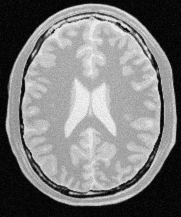
\includegraphics[width=0.3\textwidth]{../images/itk/BrainProtonDensitySlice.png}
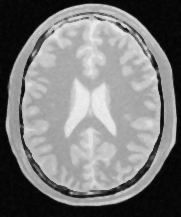
\includegraphics[width=0.3\textwidth]{../images/itk/BrainProtonDensitySliceMedian.png}

\includegraphics[width=0.3\textwidth]{../images/itk/BrainProtonDensitySliceCanny.png}
\caption{From left to right: MRI brain image, median filter, edge detection filter}
\label{fig.itk.brim}
\end{figure}

For each one of these tasks, the image analysis community has developed a
variety of algorithms, and continue developing new ones. Why do they
continue doing this?, you may ask, and the answer is that image processing is
a combination of science, engineering, art, and ``cooking'' skills. Claiming
that there is an algorithmic combination that is the ``right'' answer to an
image processing task is as misleading as claiming that there is such a thing as
the ``right'' type of chocolate dessert for a dinner. Instead of pursuing
perfection, the community strives to produce a rich set of tools that
ensures that there will be no shortage of options to try when 
facing a given image processing challenge. This state of
affairs, of course, comes at a price. The cost is that the image
analyst has the difficult task of choosing among dozens of different
tools that can be used in different combinations to achieve similar
results.

The image analysis community is closely integrated with the research
community. It is common to find that specific research groups become attached
to the algorithmic families they have developed. This custom of ``branding'',
and up to some level ``marketing'', leads to a situation where the best that the
software toolkit can do for the community is to offer a very complete set of
algorithmic implementations that they can try, and then mix and match to create
a recipe that satisfies their needs.

These are some of the reasons why ITK was designed and implemented as a large
collection of somewhat independent but coherent tools, the \emph{image filters}, many
of which can be used to solve similar problems. In this context, a certain
level of ``redundancy''---for example, offering three different implementations of
the Gaussian filter---is not seen as a problem but as a valuable feature,
because different implementations can be used interchangeably to satisfy constraints and exploit
efficiencies with respect to image size, number of processors,
and Gaussian kernel size that might be specific to a given imaging application.

The toolkit was also conceived as a resource that grows and renews itself
continuously as new algorithms and better implementations become available,
superseding existing ones, and as new tools are developed in response to the
emerging needs of new medical imaging technologies.

Armed with this quick insight into the daily
routine of the image analysts in the ITK community, we can now dive
into the main features of the architecture:

\begin{aosaitemize}
\item Modularity
\item Data Pipeline
\item Factories
\item IO Factories
\item Streaming
\item Reusability
\item Maintainability
\end{aosaitemize}

\end{aosasect2}

\begin{aosasect2}{Modularity}
Modularity is one of the main characteristics of ITK. This is a requirement
that emerges from the way people in the image analysis community work when
solving their problems. Most image analysis problems put one or more
input images through a combination of processing filters that enhance or
extract particular pieces of information from the images. Therefore
there is no single large processing object, but rather myriad small ones.
This structural nature of the image processing problem logically implies implementing the
software as a large collection of image processing filters that can be combined
in many different ways.

It is also the case that certain types of processing filters are clustered into
families, inside which some of their implementation features can be factorized.
This leads to natural grouping of the image filters into modules and groups of
modules.

Modularity, therefore occurs at three natural levels in ITK:

\begin{aosaitemize}
\item Filter Level
\item Filter Family Level
\item Filter Family Group Level
\end{aosaitemize}

At the image filter level, ITK has a collection of about 700 filters. Given
that ITK is implemented in C++, this is a natural level at which every one of
those filters is implemented by a C++ Class following object-oriented 
design patterns.  At the filter family level, ITK groups filters together
according to the nature of the processing that they perform. For example, all
filters that are related to Fourier transforms will be put together into a
Module.  At the C++ level, Modules map to directories in the
source tree, and to libraries once the software is compiled to its
binary form. ITK has about 120 of these Modules. Each module contains:

\begin{aosaenumerate}

\item The source code of the image filters that belong to that family.

\item A set of configuration files that describe how to build the module and
list dependencies between this module and other modules.

\item The set of unit tests corresponding to each one of the filters.

\end{aosaenumerate}

\aosafigure[385pt]{../images/itk/IllustrationOfModularStructure.pdf}{Hierarchical structure of groups, modules and classes}{fig.itk.modulehierarchy}

The group level is mostly a conceptual division that has been drawn on top of
the software to help locate filters in the source tree. Groups are associated
with high-level concepts such as Filtering, Segmentation, Registration and IO.
This hierarchical structure is illustrated in
\aosafigref{fig.itk.modulehierarchy}.  ITK currently has 124 modules, which are
in turn aggregated into 13 major groups.  The modules have a variety of
different sizes. This size distribution, in bytes, is presented in
\aosafigref{fig.itk.modulesize}.

\newpage %% The first line of the below para was orphaned below the diagram --ARB

\aosafigure{../images/itk/moduleSizePlotCombined.pdf}{Size distribution of 50 largest ITK modules in KB}{fig.itk.modulesize}

The modularization in ITK also applies to a set of third-party libraries
that are not directly part of the toolkit, but that the toolkit depends upon,
and that are distributed along with the rest of the code for the convenience of
users. Particular examples of these third-party libraries are the image file
format libraries: HDF5, PNG, TIFF, JPEG and OpenJPEG among others.  The third
party libraries are highlighted here because they account for about 56 percent of the
size of ITK. This reflects the usual nature of open source applications that
build upon existing platforms. The size distribution of the third-party
libraries does not necessarily reflect the architectural organization of ITK,
since we have adopted these useful libraries just as they have been developed
upstream. However, the third-party code is distributed along with the toolkit,
and partitioning it was one of the key driving directives for the
modularization process.

The module size distribution is presented here because it is a measure of the
proper modularization of the code. One can see the modularization of the code
as a continuous spectrum that ranges from the extremes of having all the code in a
single module, the monolithic version, to partitioning the code
 in a very large collection of equally sized modules. This size
distribution was a tool used to monitor the progression of the modularization
process, particularly to ensure that no big blocks of code were left in the
same module unless true logical dependencies called for such grouping.

The modular architecture of ITK enables and facilitates:

\begin{aosaitemize}
\item Reduction and clarification of cross-dependencies
\item Adoption of code contributed by the community
\item Evaluation of quality metrics per module (for example, code coverage)
\item Building selected subsets of the toolkit
\item Packaging selected subsets of the toolkit for redistribution
\item Continued growth by progressive addition of new modules
\end{aosaitemize}
\end{aosasect2}

The modularization process made it possible to explicitly identify and
declare the dependencies between different portions of the toolkit as they were
put into modules. In many cases, this exercise revealed artificial or incorrect
dependencies that had been introduced in the toolkit over time, and that passed
unnoticed when most of the code was put together in a few large groups.

The usefulness of evaluating quality metrics per module is twofold. First, 
it makes it easier to hold developers accountable for the modules which they
maintain. Second, it makes it possible to engage in
clean-up initiatives in which a few developers focus for a short period of
time on raising the quality of a specific module. When concentrating on a small
portion of the toolkit, it is easier to see the effect of the effort and to
keep developers engaged and motivated.

To reiterate, we note that the structure of the
toolkit reflects the organization of the community and in some cases the
processes that have been adopted for the continuous growth and quality control
of the software.

\begin{aosasect2}{Data Pipeline}\label{sec.itk.datapipeline}
The staged nature of most image analysis tasks led naturally to the selection
of a Data Pipeline architecture as the backbone infrastructure for data
processing. The Data Pipeline enables:

\begin{aosaitemize}

\item \emph{Filter Concatenation:} A set of image filters can be concatenated
one after another, composing a processing chain in which a sequence of
operations are applied to the input images.

\item \emph{Parameter Exploration:} Once a processing chain is put together,
it is easy to change the parameters of any filter in the chain, and to explore
the effects that such change will have on the final output image.

\item \emph{Memory Streaming:} Large images can be managed by processing only
sub-blocks of the image at a time. In this way, it becomes possible to
process large images that otherwise would not have fit into main memory.

\end{aosaitemize}

Figures~\ref{fig.itk.pipeline} and~\ref{fig.itk.brim} have already presented a
simplified representation of a data pipeline from the image processing point of
view. Image filters typically have numeric parameters that are used to
regulate the behavior of the filter. Every time one of the numeric
parameters is modified, the data pipeline marks its output as ``dirty'' and
knows that this particular filter, and all the downstream ones that use its
output, should be executed again. This feature of the pipeline facilitates the
exploration of  parameter space while using a minimum amount of
processing power for each instance of an experiment.

The process of updating the pipeline can be driven in such a way that only
sub-pieces of the images are processed at a time. This is a mechanism necessary
to support the functionality of streaming. In practice, the process is
controlled by the internal passing of a \code{RequestedRegion} specification
from one filter downstream to its provider filter upstream. This communication
is done through an internal API and it is not exposed to the application
developers. 

For a more concrete example, if a Gaussian blur image filter is
expecting to use as input a 100x100-pixel image that is produced by a median
image filter, the blur filter can ask the median filter to produce only a
quarter of the image, that is, an image region of size 100x25 pixels.  This
request can be further propagated upstream, with the caveat that every
intermediate filter may have to add an extra border to the image region size in
order to produce that requested output region size.
There is more on data streaming in \aosasecref{sec.itk.streaming}.

Both a change in the parameters of a given filter, or a change in the
specific requested region to be processed by that filter, will have the
effect of marking the pipeline as ``dirty'' and indicating the need for
a reexecution of that filter through the downstream filters in the pipeline.

\begin{aosasect3}{Process and Data Objects}

Two main types of objects were designed to hold the basic structure of the
pipeline.  They are the \code{DataObject} and the \code{ProcessObject}. The
\code{DataObject} is the abstraction of classes that carry data; for example,
images and geometrical meshes. The \code{ProcessObject} provides an abstraction
for the image filters and mesh filters that process such data.
\code{ProcessObject}s take \code{DataObject}s as input and perform some type of
algorithmic transformation on them, such as the ones illustrated in
\aosafigref{fig.itk.brim}.

\code{DataObject}s are generated by \code{ProcessObject}s. This chain typically starts by
reading a \code{DataObject} from disk, for example by using a \code{ImageFileReader} which is
a type of \code{ProcessObject}. The \code{ProcessObject} that created a given \code{DataObject} is
the only one that should modify such \code{DataObject}. This output \code{DataObject} is
typically connected as input to another \code{ProcessObject} downstream in the pipeline.

\aosafigure{../images/itk/ProcessObjectDataObject.pdf}{Relationship between \code{ProcessObject}s and \code{DataObject}s}{fig.itk.processobjectdataobject}

This sequence is illustrated in \aosafigref{fig.itk.processobjectdataobject}.
The same \code{DataObject} may be passed as input to multiple
\code{ProcessObject}s, as it is shown in the figure, where the \code{DataObject}
is produced by the file reader at the beginning of the pipeline.
In this particular case, the file reader is an instance of the
\code{ImageFileReader} class, and the \code{DataObject} that it produces as
output is an instance of the \code{Image} class.
It is also common for some filters to require two \code{DataObject}s as input,
as it is the case of the subtract filter indicated in the right side of
the same figure.

The \code{ProcessObject}s and \code{DataObject}s are connected together as a
side effect of constructing the pipeline. From the
application developer's point of view, the pipeline is linked together by
invoking a sequence of calls involving the \code{ProcessObject}s such as:

\begin{verbatim}
writer->SetInput( canny->GetOutput() );
canny->SetInput( median->GetOutput() );
median->SetInput( reader->GetOutput() );
\end{verbatim}

Internally, however, what is connected as a consequence of these calls is
not one \code{ProcessObject} to the next \code{ProcessObject}, but the
downstream \code{ProcessObject} to the \code{DataObject} that is produced by
the upstream \code{ProcessObject}.

The internal chained structure of the pipeline is held together by three types
of connections:

\begin{aosaitemize}
\item The \code{ProcessObject} holds a list of pointers to its output
\code{DataObject}s. Output \code{DataObject}s are owned and controlled by the
\code{ProcessObject} that produces them.
\item The \code{ProcessObject} holds a list of pointers to its input
\code{DataObject}s. Input \code{DataObject}s are owned by the upstream
\code{ProcessObject}.
\item The \code{DataObject} holds a pointer to its producer
\code{ProcessObject}. That happens to be the \code{ProcessObject} that also
owns and control this \code{DataObject}.
\end{aosaitemize}


This collection of internal links is later exploited to propagate calls
upstream and downstream in the pipeline. During all these interactions, the
\code{ProcessObject} retains control and ownership of the \code{DataObject}
that it generates.  The filters downstream gain access to the information about a
given \code{DataObject} through the pointer links that are established as a
consequence of the calls to the \code{SetInput()} and \code{GetOutput()} methods,
without ever taking control of that input data. For practical purposes, filters
should treat their input data as read-only objects. This is enforced in the API
by using the C++ \code{const} keyword in the arguments of \code{SetInput()}
methods. As a general rule, ITK embraces a const-correct external API, even
though internally this const-correctness is overridden by some of the pipeline
operations.

\end{aosasect3}

\begin{aosasect3}{The Pipeline Class Hierarchy}

\aosafigure[250pt]{../images/itk/ProcessObjectDataObjectHierarchy.pdf}{Hierarchy of \code{ProcessObject}s and \code{DataObject}s}{fig.itk.processobjectdataobjecthierarchy}

The initial design and implementation of the Data Pipeline in ITK was derived
from the Visualization Toolkit (VTK)\footnote{See \emph{The Architecture
of Open Source Applications}, Volume 1},  a mature project at the time
when ITK development began.

\aosafigref{fig.itk.processobjectdataobjecthierarchy} shows the object-oriented
hierarchy of the pipeline objects in ITK. In particular, note the relationship
between the basic \code{Object}, \code{ProcessObject}, \code{DataObject}, and
some of the classes in the filter family and the data family. In this
abstraction, any object that is expected to be passed as input to a filter, or
to be produced as output by a filter, must derive from the \code{DataObject}. All
filters that produce and consume data are expected to derive from the
\code{ProcessObject}. The data negotiations required to move data through the
pipeline are implemented partly in the \code{ProcessObject} and partly in the
\code{DataObject}.

The \code{LightObject} and \code{Object} classes are above the
dichotomy of the \code{ProcessObject} and \code{DataObject}. The
\code{LightObject} and \code{Object} classes provide common
functionalities such as the API for communications of \code{Events},
and the support for multi-threading.

\end{aosasect3}


\begin{aosasect3}{The Inner Workings of the Pipeline}

\aosafigref{fig.itk.processobjectdataobjectinteractionuml} presents a UML
sequence diagram describing the interactions between \code{ProcessObject}s and
\code{DataObject}s in a minimal pipeline composed of an \code{ImageFileReader},
\code{MedianImageFilter} and \code{ImageFileWriter}. 

The full interaction consist of four passes:

\begin{aosaitemize}
\item Update Output Information (upstream call sequence)
\item Update Requested Region (upstream call sequence)
\item Update Output Data (upstream call sequence)
\item Generate Data (downstream call sequence)
\end{aosaitemize}

\aosafigure[370pt]{../images/itk/ProcessObjectDataObjectInteractionUML.pdf}{UML
sequence diagram}{fig.itk.processobjectdataobjectinteractionuml}

The whole process is triggered when an application invokes the \code{Update()}
method in the last filter of the pipeline; in this concrete example this is
the \code{ImageFileWriter}. The \code{Update()} call initiates the first pass
that goes in the upstream direction. That is, from the last filter in the
pipeline, towards the first filter in the pipeline.

The goal of this first pass is to ask the question, ``How much data can
you generate for me?'' This question is codified in the method
\code{UpdateOutputInformation()}. In this method, every filter computes the
amount of image data that can be produced as output with the given amount of
data available to it as input. Given that the amount of data input must be
known first before the filter can answer the question about the amount of data
output, the question has to propagate to the filter upstream, until it reaches
a source filter that can answer the first question by itself. In this concrete
example, that source filter is the \code{ImageFileReader}. This filter can
figure out the size of its output by gathering information from the image file
that it has been assigned to read. Once the first filter of the pipeline
answers the question, then the subsequent filters downstream can compute their
respective amount of output one after another, until they make it to the last
filter of the pipeline.

The second pass, which also travels in the upstream direction, informs
filters as to the amount of output that they are requested to
produce during pipeline execution. The concept of \emph{Requested Region} is essential
in supporting the streaming capabilities of ITK. It makes it possible to tell the
filters in the pipeline not to generate the entire full image, but to focus
instead in a subregion of the image, the Requested Region. This is
very useful when the image at hand is larger than the RAM available in
the system. The call propagates from the last filter to the first one, and at
every intermediate filter the requested region size is modified to
take into account any extra borders that a filter may need in the input so it can
generate a given region size as output. In our concrete example, the
median filter will typically have to add a 2-pixel border to the size of its
own input. That is, if the writer requests a region of size 500 x 500 pixels to
the median filter, the median filter in its turn will request a region of 
502 x 502 pixels to the reader, because the median filter by default needs a
3 x 3 pixel neighborhood region to compute the value of one output pixel. The pass is
encoded in the \code{PropagateRequestedRegion()} method.

The third pass is intended to trigger the computation on the data inside the
Requested Region. This pass also goes in the upstream direction and
it is codified in the \code{UpdateOutputData()} method.  Since every filter
needs its input data before it can compute its output data, the call is passed
to the respective upstream filter first, hence the upstream propagation. Upon
return the current filter actually proceeds to computes its data.

The fourth and final pass proceeds downstream, and consists of the actual
execution of computation by every filter. The call is codified in the
\code{GenerateData()} method. The downstream direction is not a consequence
of one filter making calls on its downstream partner, but rather of the fact that the 
\code{UpdateOutputData()} calls are executing in order from the
first filter to the last filter. That is, the sequence happens downstream due
to timing of the calls, and not due to what filter is driving the calls. This
clarification is important because the ITK pipeline is by nature a \emph{Pull
Pipeline}, in which data is requested from the end, and the logic is also
controlled from the end.

\end{aosasect3}

\end{aosasect2}

\begin{aosasect2}{Factories}

One of the fundamental design requirements of ITK is to provide support for
multiple platforms. This requirement emerges from the desire to maximize the
impact of the toolkit by making it usable to a broad community regardless of
their platform of choice. ITK adopted the \emph{Factory} design pattern to
address the challenge of supporting fundamental differences among the many
hardware and software platforms, without sacrificing the fitness of a
solution to each one of the individual platforms.

The Factory pattern in ITK uses class names as keys to a registry of class
constructors. The registration of factories happens at run time, and can be
done by simply placing dynamic libraries in specific directories that ITK
applications search at start-up time. This last feature provides a natural
mechanism for implementing a plugin architecture in a clean and transparent
way. The outcome is to facilitate the development of extensible image analysis
applications, satisfying the need to provide an ever-growing set of
image analysis capabilities.

\end{aosasect2}

\begin{aosasect2}{IO Factories}
The factory mechanism is particularly important when performing IO.

\begin{aosasect3}{Embracing Diversity with Facades}

The image analysis community has developed a very large set of file formats to
store image data. Many of these file formats are designed and implemented with
specific uses in mind, and therefore are fine-tuned to specific types of
images. As a consequence, on a regular basis, new image file formats are
conceived and promoted across the community. Aware of this situation, the ITK
development team designed an IO architecture suitable for ease of
extensibility, in which it is easy to add support for more and more file
formats on a regular basis.

\aosafigure[300pt]{../images/itk/ImageIOFactoriesDesignPattern.pdf}{IO Factories dependencies}{fig.itk.io.factoriesregistry}

This IO extensible architecture is built upon the Factory mechanism
described in the previous section. The main difference is that in the case of IO,
the IO Factories are registered in a specialized registry that is managed by
the \code{ImageIOFactory} base class, shown on the upper left corner of
\aosafigref{fig.itk.io.factoriesregistry}. The actual functionality of reading
and writing data from image file formats is implemented in a family of
\code{ImageIO} classes, shown on the right side of
\aosafigref{fig.itk.io.factoriesregistry}. These service classes are intended
to be instantiated on demand when the user requests to read or write an image.
The service classes are not exposed to the application code. Instead,
applications are expected to interact with the facade classes:

\begin{aosaitemize}
\item \code{ImageFileReader}
\item \code{ImageFileWriter}
\end{aosaitemize}

\noindent These are the two classes with which the application will invoke code such as:

\begin{verbatim}
reader->SetFileName(``image1.png'');
reader->Update();
\end{verbatim}

\noindent or

\begin{verbatim}
writer->SetFileName(``image2.jpg'');
writer->Update();
\end{verbatim}

\noindent In both cases the call to \code{Update()} triggers the execution of the
upstream pipeline to which these \code{ProcessObject}s are connected. Both the
reader and the writer behave as one filter more in a pipeline. In the
particular case of the reader, the call to \code{Update()} triggers the reading
of the corresponding image file into memory. In the case of the writer, the
call to \code{Update()} triggers the execution of the upstream pipeline that is
providing the input to the writer, and finally results in an image being
written out to disk into a particular file format.

These facade classes hide from the application developer the
internal differences that are inherent to the particularities of
each file format. They even hide the existence of the file format
itself. The facades are designed in such a way that most of the
time application developers do not need to know what file formats
are expected to be read by the application. The typical
application will simply invoke code such as

\begin{verbatim}
std::string filename = this->GetFileNameFromGUI();
writer->SetFileName( filename );
writer->Update();
\end{verbatim}

\noindent These calls will work fine regardless of whether the content of the
\code{filename} variable is any of the following strings:

\begin{aosaitemize}
\item image1.png
\item image1.jpeg
\item image1.tiff
\item image1.dcm
\item image1.mha
\item image1.nii
\item image1.nii.gz
\end{aosaitemize}

\noindent where the file name extensions identify a different image file
format in every case.

\end{aosasect3}

\begin{aosasect3}{Know Thy Pixel Type}

Despite the assistance that the file reader and writer facades provide, it is
still up to the application developer to be aware of the pixel type that the
application needs to process. In the context of medical imaging, it is
reasonable to expect that the application developer will know whether the input
image will contain a MRI, a mammogram or a CT scan, and therefore be mindful of
selecting the appropriate pixel type and image dimensionality for each one of
these different image modalities. This specificity of image type might not be
convenient for application settings where users wants to read \emph{any}
image type, which are most commonly found in the scenarios of rapid prototyping
and teaching.  In the context of deploying a medical image application for
production in a clinical setting, however, it is expected that the pixel type
and dimension of the images will be clearly defined and specified based on the
image modality to be processed. A concrete example, where an application manages 3D MRI scans, looks like:

\begin{verbatim}
typedef itk::Image< signed short, 3 >  MRImageType;
typedef itk::ImageFileWriter< MRImageType > MRIWriterType;
MRIWriterType::Pointer writer = MRIWriterType::New();
writer->Update();
\end{verbatim}

There is a limit, however, to how much the particularities of the image file
formats can be hidden from the application developer.  For example, when
reading images from DICOM files, or when reading RAW images, the application
developer may have to insert extra calls to further specify the characteristics
of the file format at hand. DICOM files will be the most commonly found in
clinical environments, while RAW images are still a necessary evil for
exchanging data in the research environment.

\end{aosasect3}

\begin{aosasect3}{Together But Separate}

The self-contained nature of every IO Factory and ImageIO service class is
also reflected in the modularization. Typically, an ImageIO class depends on a
specialized library that is dedicated to managing a specific file format. That
is the case for PNG, JPEG, TIFF and DICOM, for example. In those cases, the
third-party library is managed as a self-contained module, and the specialized
ImageIO code that interfaces ITK to that third-party library is also put in a
module by itself. In this way, specific applications may disable many
file formats that are not relevant to their domain, and can focus on offering
only those file formats that are useful for the anticipated scenarios of that
application.

Just as with standard factories, the IO factories can be loaded at
run-time from dynamic libraries. This flexibility facilitates the use of
specialized and in-house developed file formats without requiring all such file
formats to be incorporated directly into the ITK toolkit itself. The loadable
IO factories has been one of the most successful features in the architectural
design of ITK. It has made it possible to easily manage a challenging situation
without placing a burden on the code or obscuring its implementation. More
recently, the same IO architecture has been adapted to manage the process of
reading and writing files containing spatial transformations represented by the
\code{Transform} class family.

\end{aosasect3}

\end{aosasect2}

\begin{aosasect2}{Streaming}\label{sec.itk.streaming}

ITK was initially conceived as a set of tools for processing the images
acquired by the Visible Human
Project\footnote{\url{http://www.nlm.nih.gov/research/visible/visible_human.html}}.
At the time, it was clear that such a large dataset would not fit in the RAM of
computers that were typically available to the medical imaging research
community. It is still the case that the dataset will not fit in the typical
desktop computers that we use today. Therefore, one of the requirements for
developing the Insight Toolkit was to enable the streaming of image data
through the data pipeline. More specifically, to be able to process large
images by pushing sub-blocks of the image throughout the data pipeline, and then
assembling the resulting blocks on the output side of the pipeline.

%% NB: This brownish grey and greenish grey is just going to end up as grey in the 
%% book --ARB
\aosafigure{../images/itk/StreamingImageDiagram.pdf}{Illustration of image streaming process}{fig.itk.streaming}

This partitioning of the image domain is illustrated in
\aosafigref{fig.itk.streaming} for the concrete example of a median filter. The
median filter computes the value of one output pixel as the statistical median
of the pixel values from the input image in a neighborhood around the
pixel. The size of that neighborhood is a numerical
parameter of the filter. In this case we set it to 2 pixels, which means
that we will take a neighborhood with a 2-pixel radius around our
output pixel. This leads to a neighborhood of 5x5 pixels with the
position of the output pixel in the middle, and a rectangular border of 2
pixels around it. This is usually called a Manhattan radius. When the median
filter is asked to computed a particular Requested Region of the
output image, it turns around and asks its upstream filter to provide a
larger region that is formed by the Requested Region enlarged by a
border of, in this case, 2 pixels.
In the specific case of \aosafigref{fig.itk.streaming}, when asked
for Region 2, of size 100x25 pixels, the median filter passes along
that request to its upstream filter for a region of size 100x29 pixels. The 29-pixel 
size in the vertical direction is computed as 25 pixels plus two borders
of 2-pixel radius each. Note that the horizontal dimension is not enlarged in
this case because it is already at the maximum that the input image can
provide; therefore, the enlarged request of 104 pixels (100
pixels plus two borders of 2 pixels) gets cropped to the maximum size of
the image, which is 100 pixels in the horizontal dimension.

ITK filters that operate on neighborhoods will take care of the boundary
conditions by using one of the three typical approaches: considering a null
value outside of the image, mirroring the pixels' values across the border, or
repeating the border value on the outside. In the case of the median filter, a
zero-flux Neumann boundary condition is used, which simply means that the
pixels outside of the region border are assumed to be a repetition of the pixel
values found in the last pixels inside the border. 

It is a well-kept dirty little
secret of the image processing literature that most of the implementation
difficulties with image filters are related to proper management of boundary
conditions. This is a particular symptom of the disconnection between the
theoretical training found in many textbooks and the software practice of image
processing.  In ITK this was managed by implementing a collection of image
iterator classes and an associated family of boundary condition calculators.
These two helper classes families hide from image filters the
complexities of managing boundary conditions in N-dimensions.

The streaming process is driven from outside the filter, typically by the
\code{ImageFileWriter} or the \code{StreamingImageFilter}. These two classes
implement the streaming functionality of taking the total size of the image
and partitioning it into a number of divisions requested by the application
developer.  Then, during their \code{Update()} call, they go in an iteration
loop asking for each one of the intermediate pieces of the image. At that
stage, they take advantage of the \code{SetRequestedRegion()} API described in
\aosafigref{fig.itk.processobjectdataobjectinteractionuml} in
\aosasecref{sec.itk.datapipeline}. That constrains the
computation of the upstream pipeline to a subregion of the image.

The application code driving the streaming process looks like

\begin{verbatim}
median->SetInput( reader->GetOutput() );
median->SetNeighborhoodRadius( 2 );
writer->SetInput( median->GetOutput() );
writer->SetFileName( filename );
writer->SetNumberOfStreamDivisions( 4 );
writer->Update();
\end{verbatim}

\noindent where the only new element is the \code{SetNumberOfStreamDivisions()} call
that defines the number of pieces into which the image will be split for the
purpose of streaming it through the pipeline. To match the example of
\aosafigref{fig.itk.streaming} we have used  four as the number of regions to
split the image into. This means that the \code{writer} is going to trigger the
execution of the \code{median} filter four times, each time with a different
Requested Region.

There are interesting similarities between the process of streaming
and the process of parallelizing the execution of a given filter. Both
of them rely on the possibility of dividing the image processing work
into image chunks that are processed separately. In the streaming
case, the image chunks are processed across time, one after another,
while in the parallelization case the image chunks are assigned to
different threads, which in turn are assigned to separate processor
cores. At the end, it is the algorithmic nature of the filter
that will determine whether it is possible to split the output
image into chunks that can be computed independently based on a
corresponding set of image chunks from the input image. In ITK,
streaming and parallelization are actually orthogonal, in the sense
that there is an API to take care of the streaming process, and a
separate API dedicated to support the implementation of parallel
computation base on multiple-threads and shared memory.

Streaming, unfortunately, can not be applied to all types of algorithms. Specific
cases that are not suitable for streaming are:

\begin{aosaitemize}
\item Iterative algorithms that, to compute a pixel value at every iteration,
require as input the pixel values of its neighbors. This is the case for
most PDE-solving-based algorithms, such as anisotropic diffusion, demons
deformable registration, and dense level sets.
\item Algorithms that require the full set of input pixel values in order to
compute the value of one of the output pixels. Fourier transform and Infinite
Impulse Response (IIR) filters, such as the Recursive Gaussian filter, are
examples of this class.
\item Region propagation or front propagation algorithms in which the
modification of pixels also happens in an iterative way but for which the
location of the regions or fronts can not be systematically partitioned in
blocks in a predictable way. Region growing segmentation, sparse level sets,
some implementations of mathematical morphology operations and some forms of
watersheds are typical examples here.
\item Image registration algorithms, given that they require access to
the full input image data for computing metric values at every iteration of
their optimization cycles.
\end{aosaitemize}

Fortunately, on the other hand, the data pipeline structure of ITK enables
support for streaming in a variety of transformation filters by taking
advantage of the fact that all filters create their own output, and therefore
they do not overwrite the memory of the input image. This comes at the price of
memory consumption, since the pipeline has to allocate both the input and
output images in memory simultaneously. Filters such as flipping, axes
permutation, and geometric resampling fall in this category. In these cases,
the data pipeline manages the matching of input regions to output regions by
requiring that every filter provide a method called
\code{GenerateInputRequestedRegion()} that takes as an argument a rectangular
output region. This method computes the rectangular input region that will be
needed by this filter to compute that specific rectangular output region. This
continuous negotiation in the data pipeline makes it possible to associate, for every
output block, the corresponding section of input image that is required for
computation.

To be more precise here, we must say therefore that ITK supports
streaming---but only in algorithms that are ``streamable'' in
nature. That said, in the spirit of being progressive regarding the remaining
algorithms, we should qualify this statement not by claiming that ``it is
impossible to stream such algorithms'', but rather that ``our typical
approach to streaming is not suitable for these algorithms'' at this point, and
that hopefully new techniques will be devised by the community in the future to
address these cases.
\end{aosasect2}

\end{aosasect1}

\begin{aosasect1}{Lessons Learned}

\begin{aosasect2}{Reusability}
The principle of reusability can also be read as ``avoidance of redundancy''.
In the case of ITK, this has been achieved with a three-pronged approach.

\begin{aosaitemize}
\item First, the adoption of object-oriented programming, and in particular the
proper creation of class hierarchies where common functionalities are
factorized in base classes.
\item Second, the adoption of generic programming, implemented via the heavy
use of C++ templates, factorizing behaviors that are identified as patterns.
\item Third, the generous use of C++ macros has also permitted reuse of standard
snippets of code that are needed in myriad places across the toolkit.
\end{aosaitemize}

Many of these items may sound like platitudes and appear obvious 
today, but when ITK development started in 1999 some of them were not that
obvious. In particular, at the time the support most C++ compilers offered
for templates did not quite follow a consistent standard. Even today,
decisions such as the adoption of generic programming and the use of a widely
templated implementation continue to be controversial in the community. This is
manifested in the communities that prefer to use ITK via the wrapping layers to
Python, Tcl or Java.


\begin{aosasect3}{Generic Programming}

The adoption of generic programming was one of the defining implementation
features of ITK. It was a difficult decision in 1999 when the 
compiler support for C++ templates was rather fragmented, and the Standard Template
Library (STL) was still considered a bit exotic.

Generic programming was adopted in ITK by embracing the use of C++ templates
for implementing generalization of concepts and in this way increasing code
reuse. The typical example of C++ template parameterization in ITK is the
\code{Image} class, that can be instantiated in the following way:

\begin{verbatim}
typedef unsigned char PixelType;
const unsigned int Dimension = 3;
typedef itk::Image< PixelType, Dimension > ImageType;
ImageType::Pointer image = ImageType::New();
\end{verbatim}

In this expression, the application developer chooses the type to be used to
represent pixels in the image, as well as the dimension of the image as a grid
in space. In this particular example, we chose to use an \code{8-bit} pixel
represented in an \code{unsigned char} type, for a 3D image. Thanks to the
underlying generic implementation, it is possible to instantiate images
of any pixel type and any dimension in ITK.

To make it possible to write these expressions, ITK developers had to implement
the \code{Image} class by being very careful with the assumptions made about
the pixel type.  Once the application developer has instantiated the image
type, the developer can create objects of that type, or proceed to instantiate
image filters whose types, in turn, depend on the image type.  For example:

\begin{verbatim}
typedef itk::MedianImageFilter< ImageType, ImageType> FilterType;
FilterType::Pointer median = FilterType::New();
\end{verbatim}

The algorithmic specificity of different image filters restricts the actual
pixel types that they can support. For example, some image filters expect the
image pixel type to be an integer scalar type while some other filters expect the pixel
type to be a vector of floating point numbers. When instantiated with inappropriate pixel
types, these filters will produce compilation errors or will result in
erroneous computational results. To prevent incorrect instantiations and to
facilitate the troubleshooting of compilation errors, ITK adopted the use of
\emph{concept checking} that is based on forcing the exercise of certain
expected features of the types, with the goal of producing early failures
combined with human-readable error messages.

C++ templates are also exploited in certain sections of the toolkit in the form
of Template Metaprogramming, with the goal of increasing run-time speed
performance of the code, in particular for unrolling loops that control the
computation of low-dimensional vectors and matrices. Ironically, we have found
over time that certain compilers have become smarter at figuring out when to
unroll loops, and no longer need the help of Template MetaProgramming
expressions in some cases.

\end{aosasect3}

\begin{aosasect3}{Knowing When to Stop}

There is also the general risk of doing ``too much of a good thing'',
meaning, there is a risk of overusing templates, or overusing macros. It is 
easy to go overboard and end up creating a new
language on top of C++ that is essentially based on the use of templates and
macros. This is a fine line, and it demands continuous attention from the
development team to make sure that the language features are properly used
without being abused.

As a concrete example, the widespread use of explicitly naming types via C++
\code{typedefs} has proved to be particularly important. This practice plays two
roles: on the one hand it provides a human-readable informative name describing the
nature of the type and its purpose; on the other hand, it ensures that the type
is used consistently across the toolkit. As an example, during the refactoring
of the toolkit for its 4.0 version, a massive effort was invested in collecting
the cases where C++ integer types such as \code{int}, \code{unsigned int},
\code{long} and \code{unsigned long} were used and to
replace them with types named after the proper concept that the associated
variables were representing. This was the most costly part of the task of
ensuring that the toolkit was able to take advantage of 64-bit types for
managing images larger than four gigabytes in all platforms. This task was of the
utmost importance for promoting the use of ITK in the fields of microscopy and
remote sensing, where image of tens of gigabytes in size are common.

\end{aosasect3}

\end{aosasect2}

\begin{aosasect2}{Maintainability}
The architecture satisfies the constraints that minimize maintenance cost.

\begin{aosaitemize}
\item Modularity (at the class level)
\item Many small files 
\item Code reuse
\item Repeated patterns
\end{aosaitemize}

\end{aosasect2}

\noindent These characteristics reduce maintenance cost in the following ways:

\begin{aosaitemize}
\item Modularity (at the class level) makes it possible to enforce test-driven 
development techniques at the image filter level, or in general
the ITK class level. Stringent testing discipline applied to small
and modular pieces of code has the advantage of reducing the pools of
code where bugs can hide, and with the natural decoupling that results
from modularization, it is a lot easier to locate defects and
eliminate them.
\item Many small files facilitate the assignment of portions of the
code to specific developers, and simplify the tracking of defects when
they are associated with specific commits in the revision control
system. The discipline of keeping small files also leads to the
enforcement of the golden rule of functions and classes: Do one
thing, and do it right.
\item Code reuse: When code is reused (instead of being copy-pasted
and reimplemented) the code itself benefits from the higher level of
scrutiny that results from being exercised in many different
circumstances. It leads more eyes to look at the code, or
at least at the effects of the code, and so the code benefits from Linus's Law:
``Given enough eyeballs, all bugs are shallow.''
\item Repeated patterns simplify the work of maintainers, who in reality 
account for more than 75\% of the cost of
software development over the lifetime of a project. Using
coding patterns that are consistently repeated in different places in
the code makes it a lot easier for a developer to open a file and
quickly understand what the code is doing, or
what it is intended to do.
\end{aosaitemize}

As the developers got involved in regular maintenance activities they
were exposed to some ``common failures'', in particular:

\begin{aosaitemize}
\item Assumptions that some filters make regarding specific pixel types for
their input or output images, but that are not enforced via types or concept
checking, and that are not specified in the documentation.
\item Not writing for readability. This is one of the most common
challenges for any software whose new algorithm implementations originate in
the research community. It is common in that environment to write code that
``just works'', and to forget that the purpose of code is not just to be
executed at run time, but to be easily read by the next
developer. Typical good rules of ``clean code'' writing---for example, write 
small functions that do one thing and one thing only (the Single Responsibility 
Principle and the Principle of Least Surprise), adhere to proper naming of variables 
and functions---tend to be ignored when
researchers are excited about getting their new shiny algorithm to work. 

\item Ignoring failure cases and error management. It is common to
focus on the ``nice cases'' of data processing and to fail to provide code for
managing all the cases that can go wrong. Adopters of the toolkit
quickly run into such cases once they start developing and deploying
applications in the real world.
\item Insufficient testing. It requires a lot of discipline to follow the
practice of test-driven development, especially the notion of writing the tests
first and only implementing functionalities as you test them. It is almost always
the case that bugs in the code are hiding behind the cases that were skipped
while implementing the testing code.
\end{aosaitemize}

Thanks to the communication practices of open source communities, many of these
items end up being exposed through questions that are commonly asked in the
mailing lists, or are directly reported as bugs by users.
After dealing with many such issues, developers learn to write code
that is ``good for maintenance''. Some of these traits apply to both coding
style and the actual organization of the code. It is our view that a developer
only reaches mastery after spending some time---at least a year---doing maintenance
and getting exposed to ``all the things that can go wrong''.

\begin{aosasect2}{The Invisible Hand}
Software should look like it was written by a single person. The best developers
are the ones who write code that, should they be hit by the proverbial bus, can 
be taken over by anybody else. We have
grown to recognize that any trace of a ``personal touch'' is an indication of a
defect introduced in the software.

In order to enforce and promote code style uniformity, the following tools have
proved to be very effective:

\begin{aosaitemize}
\item KWStyle\footnote{\url{http://public.kitware.com/KWStyle}} for automatic
source code style checking. This is a simplified C++ parser that checks coding style and
flags any violations.
\item Gerrit\footnote{\url{http://code.google.com/p/gerrit}} for regular code
reviews. This tools serves two purposes: On one hand, it prevents immature
code from entering the code base by distilling its errors, deficiencies and
imperfections during iterative review cycles where other developers contribute
to improve the code. On the other hand, it provides a virtual
training camp in which new developers get to learn from more experienced
developers (read ``experienced'' as \emph{have made all the
mistakes and know where the bodies are buried\ldots}) how to improve the
code and avoid known problems that have been observed during maintenance
cycles.
\item Git hooks that enforce the use of the KWStyle and Gerrit and that also
perform some of their own checks. For example, ITK uses Git hooks that prevent
commits of code with tabs or with trailing blank spaces.
\item The team has also explored the use of
Uncrustify\footnote{\url{http://uncrustify.sourceforge.net}} as a tool for
enforcing a consistent style.
\end{aosaitemize}

It is worth emphasizing that uniformity of style is not a simple matter of
aesthetic appeal, it is really a matter of economics.
Studies on the \emph{Total Cost of Ownership} (TCO) of software projects have
estimated that in the life-cycle of a project, the cost of maintenance will be
about 75\% of the TCO, and given that maintenance cost is applied on an annual
basis, it typically surpasses the cost of initial development costs by the
first five years of the life-cycle of a software
project\footnote{\emph{``Software Development Cost Estimating Handbook''},
Volume I, Naval Center for Cost Analysis, Air Force Cost Analysis Agency,
2008.}. Maintenance is estimated to be about 80\% of what software developers
actually do, and when engaged in that activity the large majority of the
developer's time is dedicated to reading someone else's code, trying to figure
out what it was supposed to do\footnote{\emph{``Clean Code, A Handbook of
Agile Software Craftsmanship''}, Robert C.  Martin, Prentice Hall, 2009}.
Uniform style does wonders for reducing the time it takes for developers to
immerse themselves in a newly open source file and understand the code before
they make any modifications to it.  By the same token, it reduces the chances
that developers will misinterpret the code and make modifications
that end up introducing new bugs when they were honestly trying to fix old
bugs\footnote{\emph{``The Art of Readable Code''}, Dustin Boswell, Trevor
Foucher, O'Reilly, 2012}.

The key for making these tools effective is to make sure that they are:
\begin{aosaitemize}
\item Available to all developers, hence our preference for Open Source tools.
\item Run on a regular basis. In the case of ITK, these tools have been
integrated in the Nightly and Continuous Dashboard builds managed by
CDash\footnote{\url{http://www.cdash.org/CDash/index.php?project=Insight}}.
\item Run as close as possible to the point where the code is being written,
so that deviations can be fixed immediately, and so developers
quickly learn what kind of practices break style rules.
\end{aosaitemize}

\end{aosasect2}

\begin{aosasect2}{Refactoring}
ITK started in 2000 and grew continuously until 2010. In
2011, thanks to an infusion of federal funding investment, the development team
had the truly unique opportunity to embark on a refactoring effort. The funding
was provided by the National Library of Medicine as part of the initiative of
the American Recovery and Reinvestment Act (ARRA). This was not a minor undertaking.
Imagine you have been working on a piece of software for over a decade, and you
are offered the opportunity to clean it up; what would you change?

This opportunity for widespread refactoring is very rare. For the previous ten
years, we had relied on the daily effort of performing small local
refactorings, cleaning up specific corners of the toolkit as we ran into
them.  This continuous process of clean up and improvement takes advantage of
the massive collaboration of open source communities, and it is safely enabled
by the testing infrastructure driven by CDash, which regularly exercises
about 84\% of the code in the toolkit. Note that in contrast, the average
code coverage of software industry testing is estimated to be only 50\%.

Among the many things that were changed in the refactoring effort, the ones
that are most relevant to the architecture are:

\begin{aosaitemize}
\item Modularization was introduced in the toolkit
\item Integer types were standardized
\item Typedefs were fixed to allow management of images larger than 4 GB on all platforms
\item The software process was revised:
  \begin{aosaitemize2}
    \item Migrated from CVS to Git
    \item Introduced code review with Gerrit
    \item Introduced testing on demand with CDash@home
    \item Improved method for downloading data for unit testing
  \end{aosaitemize2}
\item Deprecated support for obsolete compilers
\item Improved support for many IO image file formats including:
  \begin{aosaitemize2}
    \item DICOM
    \item JPEG2000
    \item TIFF (BigTIFF)
    \item HDF5
  \end{aosaitemize2}
\item Introduced a framework for supporting GPU computation
\item Introduced support for video processing
  \begin{aosaitemize2}
    \item Added a bridge to OpenCV
    \item Added a bridge to VXL
  \end{aosaitemize2}
\end{aosaitemize}

Maintenance based on incremental modifications---tasks such as adding
features to an image filter, improving performance of a given
algorithm, addressing bug reports, and improving documentation of
specific image filters---works fine for the local improvement of specific C++ 
classes. However, a massive refactoring is needed for
infrastructure modifications that affect a large number of classes
across the board, such as the ones listed above. For example,
the set of changes needed to support images larger
than 4 GB was probably one of the largest patches ever applied to ITK.
It required the modification of hundreds of classes and could not have
been done incrementally without incurring in a great deal of pain. The
modularization is another example of a task that could not have
been done incrementally. It truly affected the entire organization of
the toolkit, how its testing infrastructure works, how testing data
is managed, how the toolkit is packaged and distributed, and how new
contributions will be encapsulated to be added to the toolkit in the
future.

\end{aosasect2}

\begin{aosasect2}{Reproducibility}

One of the early lessons learned in ITK was that the many papers published in
the field were not as easy to implement as we were led to believe.  The
computational field tends to over-celebrate algorithms and to dismiss the
practical work of writing software as ``just an implementation detail''.

That dismissive attitude is quite damaging to the field, since it diminishes the
importance of the first-hand experience with the code and its proper use. The
outcome is that most published papers are simply not reproducible, and 
when researchers and students attempt to use such techniques they end up
spending a lot of time in the process and deliver \emph{variations} of the
original work. It is actually quite difficult, in practice, to verify if an
implementation matches what was described in a paper.

ITK disrupted, for the good, that environment and restored a culture of DIY
to a field that had grown accustomed to theoretical
reasoning, and that had learned to dismiss experimental work. The new culture
brought by ITK is a practical and pragmatic one in which the virtues of the
software are judged by its practical results and not by the appearance of
complexity that is celebrated in some scientific publications. It turns
out that in practice the most effective processing methods are those that
would appear to be too simple to be accepted for a scientific paper.

The culture of reproducibility is a continuation of the philosophy of test
driven development, and systematically results in better software; higher
clarity, readability, robustness and focus.

In order to fill the gap of lack of reproducible publications, the ITK community
created the Insight Journal\footnote{\url{http://www.insight-journal.org}}.
It is an open-access, fully online publication in which contributions are
required to include code, data, parameters, and tests in order to enable
verification by reproducibility. Articles are published online less than 24
hours after submission. Then they are made available for peer-review by any
member of the community. Readers get full access to all the materials
accompanying the article, namely source code, data, parameters, and testing
scripts. The Journal has provided a productive space for sharing new code
contributions which from there make their way into the code base. The Journal
recently received its 500th article, and continues to be used as the official
gateway for new code to be added to ITK.
\end{aosasect2}

\end{aosasect1}

\end{aosachapter}
